\chapter{Align the domains}
For alignment, I used \href{http://www.genome.jp/tools/clustalw/}{Multiple Sequence Alignment by CLUSTALW}.

I chose the following options:
\begin{itemize}
\item Output Format: CLUSTAL
\item Gap Open Penalty: 10.0
\item Gap Extension Penalty: 0.05
\item No Weight Transition
\item Hydrophilic Residues for Proteins: \texttt{GPSNDQERK}
\item Weight Matrix: \textbf{BLOSUM} (for PROTEIN)
\end{itemize}

And the result is in \url{~/files/ex3clustal.aln}.

However, I have also found an opportunity to draw phylogenetic trees of the sequences provided. On Figure \ref{phytree1} a \emph{rooted 
phylogenetic tree with branch length} is depicted.
Probably the PDZ1 and the PDZ2 domain is replicated, because they are very close to each other, both in the DLG3 sequence and in \emph{code distance too}

\begin{figure}
\centering
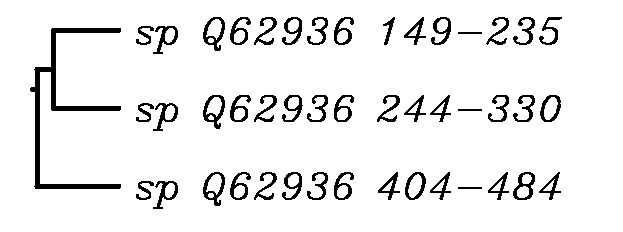
\includegraphics[width=\textwidth]{phylogenic.png}
\caption{\href{http://www.genome.jp/tools-bin/clustalwtree?treebl_upgma+1611190754597I9T9}{Source}}
\label{phytree1}
\end{figure}

